% $Id: template.tex 11 2007-04-03 22:25:53Z jpeltier $

\documentclass{vgtc}                          % final (conference style)
%\documentclass[review]{vgtc}                 % review
%\documentclass[widereview]{vgtc}             % wide-spaced review
%\documentclass[preprint]{vgtc}               % preprint
%\documentclass[electronic]{vgtc}             % electronic version

%% Uncomment one of the lines above depending on where your paper is
%% in the conference process. ``review'' and ``widereview'' are for review
%% submission, ``preprint'' is for pre-publication, and the final version
%% doesn't use a specific qualifier. Further, ``electronic'' includes
%% hyperreferences for more convenient online viewing.

%% Please use one of the ``review'' options in combination with the
%% assigned online id (see below) ONLY if your paper uses a double blind
%% review process. Some conferences, like IEEE Vis and InfoVis, have NOT
%% in the past.

%% Figures should be in CMYK or Grey scale format, otherwise, colour 
%% shifting may occur during the printing process.

%% These few lines make a distinction between latex and pdflatex calls and they
%% bring in essential packages for graphics and font handling.
%% Note that due to the \DeclareGraphicsExtensions{} call it is no longer necessary
%% to provide the the path and extension of a graphics file:
%% \includegraphics{diamondrule} is completely sufficient.
%%
\ifpdf%                                % if we use pdflatex
  \pdfoutput=1\relax                   % create PDFs from pdfLaTeX
  \pdfcompresslevel=9                  % PDF Compression
  \pdfoptionpdfminorversion=7          % create PDF 1.7
  \ExecuteOptions{pdftex}
  \usepackage{graphicx}                % allow us to embed graphics files
  \DeclareGraphicsExtensions{.pdf,.png,.jpg,.jpeg} % for pdflatex we expect .pdf, .png, or .jpg files
\else%                                 % else we use pure latex
  \ExecuteOptions{dvips}
  \usepackage{graphicx}                % allow us to embed graphics files
  \DeclareGraphicsExtensions{.eps}     % for pure latex we expect eps files
\fi%

%% it is recomended to use ``\autoref{sec:bla}'' instead of ``Fig.~\ref{sec:bla}''
\graphicspath{{figures/}{pictures/}{images/}{./}} % where to search for the images

\usepackage{microtype}                 % use micro-typography (slightly more compact, better to read)
\PassOptionsToPackage{warn}{textcomp}  % to address font issues with \textrightarrow
\usepackage{textcomp}                  % use better special symbols
\usepackage{mathptmx}                  % use matching math font
\usepackage{times}                     % we use Times as the main font
\renewcommand*\ttdefault{txtt}         % a nicer typewriter font
\usepackage{cite}                      % needed to automatically sort the references
\usepackage{tabu}                      % only used for the table example
\usepackage{booktabs}                  % only used for the table example
%% We encourage the use of mathptmx for consistent usage of times font
%% throughout the proceedings. However, if you encounter conflicts
%% with other math-related packages, you may want to disable it.


%% If you are submitting a paper to a conference for review with a double
%% blind reviewing process, please replace the value ``0'' below with your
%% OnlineID. Otherwise, you may safely leave it at ``0''.
\onlineid{0}

%% declare the category of your paper, only shown in review mode
\vgtccategory{Research}

%% allow for this line if you want the electronic option to work properly
\vgtcinsertpkg

%% In preprint mode you may define your own headline.
%\preprinttext{To appear in an IEEE VGTC sponsored conference.}

%% Paper title.

\title{Increasing Efficiency and Optimization within Virtual Keyboards}

%% This is how authors are specified in the conference style

%% Author and Affiliation (single author).
%%\author{Roy G. Biv\thanks{e-mail: roy.g.biv@aol.com}}
%%\affiliation{\scriptsize Allied Widgets Research}

%% Author and Affiliation (multiple authors with single affiliations).
\author{Nia Bennabhaktula \thanks{e-mail: pragjnab@rams.colostate.edu}\\ 
\and Aaron Lawrence \thanks{e-mail:ed.grimley@aol.com}\\ 
%\and Martha Stewart\thanks{e-mail:martha.stewart@marthastewart.com}}
\affiliation{\scriptsize Colorado State University}
}
%% Author and Affiliation (multiple authors with multiple affiliations)
%\author{Nia Bennabhaktula \thanks{e-mail: pragjnab@rams.colostate.edu}\\ %
%        \scriptsize Colorado State University %
%\and Aaron Lawrence \thanks{e-mail:ed.grimley@aol.com}\\ %
%    \scriptsize Colorado State University %


%% A teaser figure can be included as follows, but is not recommended since
%% the space is now taken up by a full width abstract.
%\teaser{
%  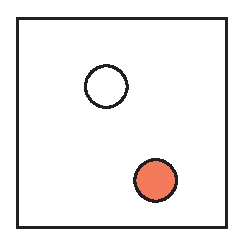
\includegraphics[width=1.5in]{sample.eps}
%  \caption{Lookit! Lookit!}
%}

%% Abstract section.
\abstract{For this project, we looked at various ways users input text into a virtual keyboard on a smart TV. Smart TV's are one of the most used and it is important to have and interactive device between user and platform that can enter and edit text effectively\cite{choi:2016}.
 We propose a potential experiment utilizing a Virtual Reality (VR) environment to test different 3 methods of interacting with a virtual keyboard that aims to improve speed and accuracy. The first way is using a button-based control method, where buttons on a remote control move a cursor around to different characters, and then input the selected one. The second way is using a motion-based pointer, which is a common way users interact with smart TV virtual keyboards. The third method is a hybrid of the other two methods, designed with hopes of increasing typing speed and accuracy for the common motion-based scheme. We also propose a survey study that would supplement this experiment and help to see how users feel about current control methods.%
} % end of abstract

%% ACM Computing Classification System (CCS). 
%% See <http://www.acm.org/class/1998/> for details.
%% The ``\CCScat'' command takes four arguments.

\CCScatlist{ 
  \CCScat{Optimization of Virtual Keyboards}%
{Virtual Reality}{QWERTY};
  \CCScat{Keyboards}
}

%% Copyright space is enabled by default as required by guidelines.
%% It is disabled by the 'review' option or via the following command:
% \nocopyrightspace

%%%%%%%%%%%%%%%%%%%%%%%%%%%%%%%%%%%%%%%%%%%%%%%%%%%%%%%%%%%%%%%%
%%%%%%%%%%%%%%%%%%%%%% START OF THE PAPER %%%%%%%%%%%%%%%%%%%%%%
%%%%%%%%%%%%%%%%%%%%%%%%%%%%%%%%%%%%%%%%%%%%%%%%%%%%%%%%%%%%%%%%%

\begin{document}

%% The ``\maketitle'' command must be the first command after the
%% ``\begin{document}'' command. It prepares and prints the title block.

%% the only exception to this rule is the \firstsection command
\firstsection{Introduction}

\maketitle

%% \section{Introduction} %for journal use above \firstsection{..} instead
Computers have been heavily integrated in today’s world. Technology has been constantly evolving as the computing environment grows. 20 years ago, we probably would not have been able to imagine a portable computer to carry around and be used for multiple purposes. Today almost everyone has access to a laptop and has become dependable in this society. To use any computing system, the users need an input device that allows them to interact with the computer. These input devices are necessary to convert the physical aspects of the user through touch, motion, sound etc., and convert them into signals for the computer\cite{taveria:2009}.\\[1em]
One of the oldest and most commonly used computer input devices is the keyboard\cite{taveria:2009}. It is an integral part of the computer designed to let users interact with the screen. With the upgrade of technology and faster development of graphics, microprocessors and various other technologies hitting the market, its allowing users to fully immerse themselves into a different reality\cite{mazuryk:1999}. Virtual Reality (VR) presents a 4D experience and allows the users to interact with a different reality from the inside instead of seeing it on a screen. With how big keyboards are getting, more research on this topic will increase their productivity and capability amongst all devices. This paper delves into VR keyboards and studies how to increase efficiency and provide better utilization of the input device in a virtual setting. 
Physical keyboards have been primarily designed for tactile usage while virtual keyboards are behind with utilization with pointing devices\cite{topal:2012}. Because of this, virtual keyboards require more research to optimize their design and improve the modal and functional assets. Virtual keyboards such as on-screen keyboards have been used as an alternative to physical keyboards. They provide users more accessibility and reinforce security while entering data\cite{topal:2012}.

\section{Related Work}

When it comes to trying to improve text input for virtual keyboards, there are two areas that people have been focused on. To optimize virtual keyboards, analysis of entry speeds, error rates and how users learn and perform need to be taken into consideration \cite{27}.The first area is related to the virtual keyboard layouts. One study that focused on this area involved participants typing on an invisible keyboard to see how feasible more transparent virtual keyboards could be\cite{32}. Another study focused on key size, and distance from each other, to see if that could improve input speed\cite{34}. Yet another example of a study in this area focused on predictive virtual keyboards, where they would predict the next letter or word as you typed\cite{25}.\\[1em]
The second area is related to the devices users use to actually interact with the keyboards. This would include methods such as changing remote controllers to use different button layouts or different control methods, or even using an input device that is completely different from a standard remote control. This area doesn’t just focus on improving typing efficiency on virtual keyboards. A number of studies have been done to try and find more accessible control types for people with difficulties using traditional controllers, such as paralysis. A recent example of a study focused on this area was one that was conducted to try out continuous-gesture-based methods for texting where a continuous movement of the mouse was used to trace letters on the keyboard that used a predictive language model. The issue with this method was that the users had to constantly recognize the dynamically arranged letters multiple times\cite{Zhai:2002}. The experiment was done by Zhai et al., (2000).


\subsection{Why switch to Virtual Keyboards?}

With an increase of smart TV’s and smartphones, physical keyboards have become less supportive with such devices and more popular towards onscreen method\cite{13}. A recent study compares four input devices (traditional remote controller, touchpad, physical keyboard, and smart device virtual keyboard) and how well they function when typing on a smart TV. The data collected was both qualitative and quantitative measuring both efficiency and user satisfaction\cite{li:2015}. Comparing the physical keyboard and the virtual keyboard, results showed that although the physical keyboard possess speed, it is not very good to edit text on screen. The best option out of the four input devices proved to be the virtual keyboard. It showed more flexibility and user acceptance towards smart TV’s\cite{li:2015}. 
\subsection{Layout}
To increase efficiency of virtual keyboards, there have been many studies that put forward various keyboard designs that have improved speed and accuracy. A study was done to understand whether smaller keyboards have an effect on input speed. MacKenzie et al. \cite{Mackenzie:2015} showed that while using a stylus input method, a smaller sized keyboard did not affect speed negatively compared to a larger keyboard. They used the QWERTY standard keyboard layout and concluded that users switching from desktop keyboards to phones or other devices would not reduce any benefits.\\[1em]
Findlater et al. \cite{findlater:2012} designed two personalized keyboard interfaces that adapt the underlying key-press classification modals based on what the user is typing. One keyboard was designed to keep a visually stable rectangular layout while the other keyboard visually adapted according to the input. Results showed that the non-visual adaptive keyboard was more user friendly and improved typing speed while the visual adaptive keyboard was considered more natural but had a negative impact on speed \cite{findlater:2012}.
\begin{figure}[h!]
 \centering % avoid the use of \begin{center}...\end{center} and use \centering instead (more compact)
 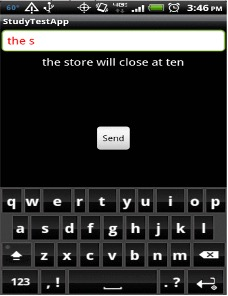
\includegraphics[width=\columnwidth]{rt.jpg}
 \caption{Real-Time keyboard}
 \label{fig:rt}
\end{figure}
\begin{figure}[h!]
 \centering % avoid the use of \begin{center}...\end{center} and use \centering instead (more compact)
 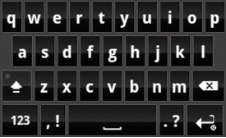
\includegraphics[width=\columnwidth]{stand.jpg}
 \caption{Standard Keyboard}
 \label{fig:standard}
\end{figure}
\begin{figure}[h!]
 \centering % avoid the use of \begin{center}...\end{center} and use \centering instead (more compact)
 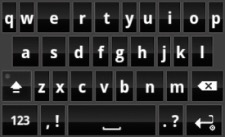
\includegraphics[width=\columnwidth]{static.jpg}
 \caption{Static Keyboard}
 \label{fig:static}
\end{figure}

Another study by Kuno et al.  \cite{kuno:2013} designed a keyboard where the key position and size automatically adjust according to the user’s hand. They used touch-based recognition to enable faster typing. Using the QWERTY layout, A, S, D, F, Space, Enter, J, K, L, and semi-colon; home position keys were places at the touch point of each finger while the non-home keys were in the surroundings. Results showed that the users were able to type faster with only a small amount of hand movement, but the focus was only on one finger touch point at a time.\cite{13} has experimented whether users are more comfortable with standard, real-time or static keyboards (see Figure 1, 2 and 3). Participants were asked to type phrases in both portrait and landscape orientations. Quantitative results showed that the QWERTY standard keyboard was the most comfortable in both portrait and landscape\cite{13}.\\[1em] 
A similar study that uses six different entry methods compares the text input methods for digital television \cite{28}. An empirical study that examines entry speeds and error rates using  devices like full-sized keyboard, a palm-sized keyboard, a gyroscopic remote point-select, and a modified touchpad \cite{28}. Although the standard keyboard showed the fastest entry rates it also had complaints of low lighting and visibility to the user. The error rates were similar for both types of keyboards and the gyroscopic method. This study suggested a new design of text entry methods that are more user friendly and contain a lower error rate. 

\begin{figure}[h!]
 \centering % avoid the use of \begin{center}...\end{center} and use \centering instead (more compact)
 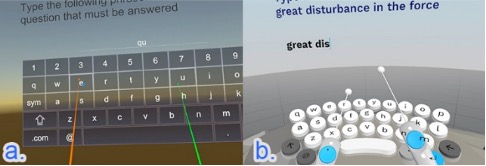
\includegraphics[width=\columnwidth]{ab.jpg}
 \caption{(a)Raycasting Keyboard (b)Drum-Like Keyboard}
 \label{fig:ab}
\end{figure}
\begin{figure}[h!]
 \centering % avoid the use of \begin{center}...\end{center} and use \centering instead (more compact)
 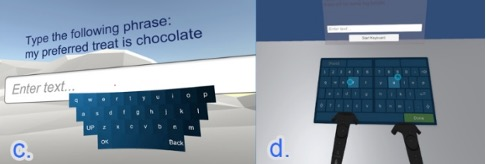
\includegraphics[width=\columnwidth]{bc.jpg}
 \caption{(c)Head-Directed Keyboard (d)Split Keyboard}
 \label{fig:cd}
\end{figure}

Another empirical study that opposes the standard keyboard layout was done by \cite{23}. Specifically using controller based text-inputs, the study tested usability and error rates. Four different VR text-input techniques were used. Figure 4 and 5 show the different inputs: (a) raycasting, (b) drum-like keyboard, (c) head-directed input, and (d) split keyboard. The drum-like keyboard showed higher rates of usability, satisfactory entry scores and moderate error rates \cite{23}. Although this new styled keyboard has moderate error rates which are higher than the standard straight layout, it was given more positive experienced feedback from users\cite{23}.

\subsection{Keyboard Design}

In most of the studies that were previously done, we see that research done using the QWERTY straight standard layout allows users to transfer the same typing skills since the layout is similar\cite{Mackenzie:2015}. This layout has shown higher levels of speed and accuracy with the lowest error rates. For this study, we would keep using the QWERTY layout but using gesture-based techniques to improve efficiency.\\[1em]
When it comes to designing a virtual keyboard that is friendly for the user, it is important to consider the sizing and spacing between the keys as well. In an attempt to create a user-friendly keyboard, a study by\cite{10} studies multiple keyboards based on size and center distance between the keys. The study shows that the typing speed is directly related with the width and distance between keys. The keyboard was designed in such a way that when the user performance did not match with the standard keyboard layout, the keyboard would adapt and modify its size and distance to enhance the typing performance\cite{10}.\cite{34} has a similar study that explores how size and spacing expansion ratio effect a motion controlled remote. Although this study is more based on motion control, its results still show that appropriate size, space, expansion ratio and location of keys allow for users to type with more ease\cite{34}.\\[1em]
Both of these studies iterate the importance of the size, width, and distance between keys as its proven to improve typing quality for users. The way a keyboard is designed can significantly improve error rate, speed, and accuracy as well. The design is essential in order to improve efficiency and optimization within VR keyboards. 
\subsection{Functions}

In most of the studies, three different categories were mainly tried inorder to optimize virtual keyboards.
\subsubsection{Eye-Tracking}

Although the touch interface Is more commonly used and has advantage towards user experience and a dynamic GUI, ouch touch interfaces still have their limitations when it comes to smart TV’s \cite{19}. To understand the full ability of virtual keyboards, research needs to be done on multiple sense-based modalities and inputs in increase efficiency and understand which method would be more useful.\\[1em]
A study done by \cite{16} proposed two different prototypes (see Figure 6) to increase user experience. Prototype A allowed users to avoid head-swinging and could scan the screen from top to bottom using their eyes, but showed disadvantage towards larger screens \cite{16} . Prototype B had distributed the buttons evenly on the screen which showed it was much more suited for larger screens such as smart TV’s \cite{16} . \\[1em]
\begin{figure}[h!]
 \centering % avoid the use of \begin{center}...\end{center} and use \centering instead (more compact)
 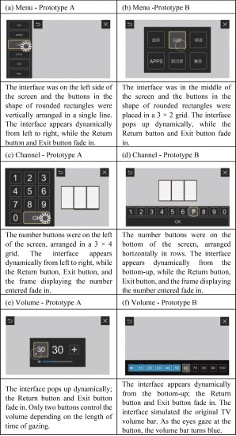
\includegraphics[width=\columnwidth]{PA.jpg}
 \caption{Prototype A and Prototype B}
 \label{fig:prototype}
\end{figure}
Based on the results the study concluded that the eye-ball tracking is highly sensitive and needs flexibility of size and sensing around to be effective \cite{16}. 
The position of the iris also matters when designing gaze-controlled input methods. A study done by  \cite{14}  designed a virtual keyboard that tracks the position of the iris using digital imaging and projects the position onto the keyboard. 
\subsubsection{Speech}

A study done by \cite{17} presents a We present a multi-modal text entry device called the SpeeG2 that combines speech recognition with gesture-based error correction \cite{17}. With an average type speed of 38 word per minute (WPM), this new prototype was able to reach till 21.04 WPM using speech \cite{17}.\\[1em]
Another study mentions voice levels to input different text entries. The prototype is designed where the pitch and volume of the voice allows the user to interact with the keyboard \cite{21}.\\[1em]
Another study used four immersive VR environments: pinch keyboards, one-hand chord keyboard, soft keyboard with a pen and tablet, and speech \cite{22}.This experiment measures performance and usability of the four different techniques.The results showed that the speech technique was the fastest but the keyboard had the fewest errors \cite{22}.
\subsubsection{Gesture}
A study done by \cite{33} examines how the users' gesture typing ability with with keyboard size and location compares to their typing performance with touch. The study improves on a design to address the uncertainty of touch based modals. The prototype they used with indirect gesture typing had a 22.3 WPM\cite{33}.\\[1em]
Similar to the above, LeapKII-GUI, which is a prototype designed by \cite{20} presents an algorithm based gesture recognition interface that allows users to use their fingertip gestures and enter text remotely \cite{20}. This protoype resulted in enhancing the speed on an analysys with typing on smart TV's \cite{20}.
The present study proposes a way of entering letters by recognizing gesture movements. \\[1em]
Another study used "frequency modulated continuous wave (FMCW) radar
with noise removal and range gating method to recognize human
hand gesture for a user moving in the radar’s field of view" \cite{39}. These gestures were used on a remote controller for a PC, the results showed that with removing noise the gesture commands like swiping left and swiping right were identified from a distance between 0.3m to 1.2m \cite{39}.

\subsection{VR Limitations}

Although VR keyboards in itself have a lot of studies focused on optimizing the performance for user experience, studies on multi-modal input access facilities for those who are visually impaired are limited \cite{12}. A study was done to optimize VR keyboards for stroke patients using eye-tracking interaction. This study was designing a Hindi keyboard that combines letter frequency and selection times in order to create a ‘gaze-controlled tree-based menu selection system’ \cite{12}. The results showed that the gaze based GUI virtual keyboard improved speed and accuracy. The experiment was done using both healthy subjects and stroke patients allowing them to compare both group which showed that stroke patients did find it much easier to type and use a keyboard  \cite{12} .\\[1em]
 \cite{11}  designed a VR keyboard that is accessed through blink-control method for those who are severely disabled. The study proposed a Bluetooth headset that detects and converts pseudo electromyography (EMG) signals of blinking to inputs for the virtual keyboard  \cite{11}. Using algorithms proposed in the study, the device used conscious blinks and different variations to activate functions within the keyboard  \cite{11}.  \\[1em]
 \cite{18}  also investigates something similar for the visually impaired. This study is concerned with people with vision impairment seeing smaller buttons and functions on the smart TV’s. To combat this issue, they use a mobile app that has modalities such as air gestures and speech commands to increase user experience \cite{18}. Results indicated that touch and speech were more effective than a remote controller\cite{18}. A study done by \cite{15} specifically determines which text entry implementation is best for VR. Results showed that the on-table virtual keyboard had higher positive feedback while mid-air gesture was neutral and ten-finger mid-air was negative \cite{18}.  \\[1em]
A study aimed towards those with speech impairments showed that a virtual keyboard was able to take inputs used from hissing sounds\cite{26}. Participants were able to input text using the speed of hissing per minute\cite{26}. These results indicate that predictability is necessary for users to enhance performance\cite{26}. 

\section{Method}

In order to determine the effectiveness of different control types, our group would perform a controlled experiment. For this experiment, we would gather 30 participants and split them equally into 3 groups of 10 participants each. Every participant would start off by being given a list of items that they would be searching for, these “items” being groups of words. The items would vary by number of characters in each word, as well as number of words. After being given the list, the participants would be put into a virtual environment. The environment would consist of a room with a TV in it. This TV would show a virtual keyboard with a search bar. The controllers would act as a remote to interact with the TV, using the movement stick to act as arrow buttons, and having a button to confirm. There would additionally be a "ready" button that starts the testing. Participants would start off being able to use the keyboard without having to search for anything in particular in order to get used to how the remote works in the virtual environment. Then, when the participants are ready, they would push the ready button. This would cause the TV to display the first item to search for, and the participant would have to try and type in what is displayed and confirm it as fast as possible. Participants would be timed in seconds and milliseconds for how fast they are able to match the items. They would have to match the items exactly to proceed, but they would also be able to delete mistakes as many times as needed. Their speeds would be recorded as they go, but not shown to the participants during the tests. After correctly inputting the correct item, the timer would pause. Once ready, the participants would push the ready button again, displaying the next item and resuming the timer. After 5 items are shown, the participant will get a longer break, during which they would be told about the next control method. After being given a chance to get used to using this new method, participants would hit the ready button to begin the next part, and the process would repeat with participants having to input 5 new items with this new control method. After participants get through these 5 items, participants would get another longer break and be told about the final control method. Once again, when the participants are ready, they would push the ready button and repeat the process of inputting one last set of 5 new items using this third control method. After finishing this last set, the trial would be finished. \\[1em]
The three control styles that participants would have to use are button based, motion based, and a hybrid of both. Button based would be using arrow buttons to move the selected key and pushing the confirm button to input it. Motion based would be pointing the remote at the keys to select them and pushing the confirm button to input it. For the hybrid control method, users would select keys by pointing the remote at them and pushing the confirm button to input them like with the motion based control style, but users could also input the keys adjacent to the selected key by pushing the arrow buttons. \\[1em]
We would take several steps to ensure that the results of the experiment were due to the variations in control methods, and not some other factor. As part of this, the virtual room the participants would be in would have 3 different teleport locations. One would be at the opposite side of the room from the TV, one would be very close to the TV, and the third would be in the middle of the two. Having these teleport spots would allow participants to choose a comfortable distance from the TV where they could clearly see as much of the screen as they need. Additionally, we would assign different groups of participants to different control styles first. One group of participants would start with the button based style, the second group would start with the motion based style, and the third group would start with the hybrid style. The order of styles would be button, motion, hybrid, button, etc. Participants would get the same set of items to search for in the same order as well. This, when combined with the different starting methods, would ensure that each set of items gets tested for all three methods.\\[1em]
After participants do all of the tests, they would be given a brief survey before they leave. This survey would ask the participants which of the methods they enjoyed using the most, which they thought was the fastest (regardless of whether it actually was or not), and if any of the control styles felt confusing. Generally, the questions would be focused on how the participants felt about each of the control styles, regardless of the actual data gathered.
After performing this study with all 30 participants, we would observe both the recorded times and the survey responses. While the times we’d gather would be important in determining the effectiveness of the different control styles, the surveys would also help us to determine the enjoyability of them as well, which our group believes is another important factor of an effective input device.
\begin{figure}[h!]
 \centering % avoid the use of \begin{center}...\end{center} and use \centering instead (more compact)
 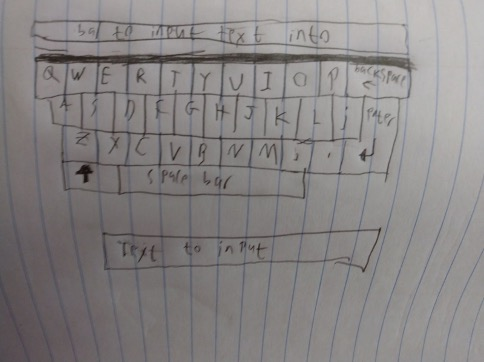
\includegraphics[width=\columnwidth]{img1.jpg}
 \caption{A visualization of the keyboard layout for remote styles}
 \label{fig:remote}
\end{figure}
Figure 7 shows sketch of keyboard layout for the remote usage styles. It is a typical QWERTY layout keyboard, with the minor difference of only having one shift key on the left side. The backspace key and enter key is on the right, the latter of which is used to confirm text input into the search bar. The search bar can be seen above the keyboard, with a thin black separator in between the two. Underneath the keyboard, there is a second bar that displays the text participants will have to enter into the search bar. \\[1em]
\begin{figure}[h!]
 \centering % avoid the use of \begin{center}...\end{center} and use \centering instead (more compact)
 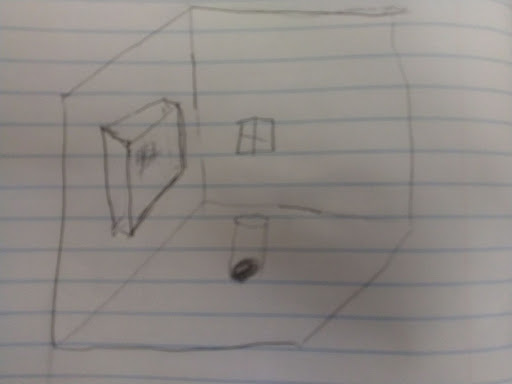
\includegraphics[width=\columnwidth]{img2.jpeg}
 \caption{Visual sketch of where the experiment will take place}
 \label{fig:room}
\end{figure}
Figure 8 is a sketch of the room participants would be in. The rectangle on the far left is the “tv”, and the cylinder in the middle represents both the starting area for the participants, and the middle teleport location. The other two teleport locations would be a few inches from the left wall, and a few inches from the right wall. There is a window in the back, and possibly multiple other cosmetic additions (chairs, tables, etc.) to make the area seem more like a house, however these aren’t necessary. \\[1em]
\begin{figure}[h!]
 \centering % avoid the use of \begin{center}...\end{center} and use \centering instead (more compact)
 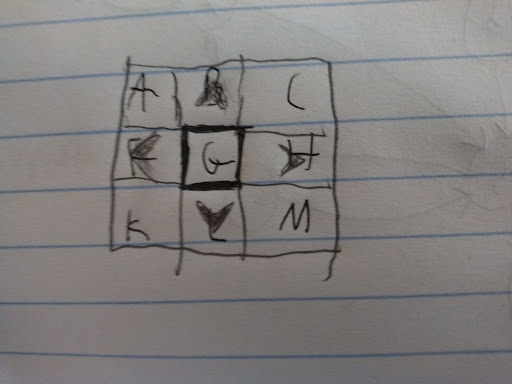
\includegraphics[width=\columnwidth]{img3.jpeg}
 \caption{Visual sketch of the arrow keys used to select method}
 \label{fig:keys}
\end{figure}
Figure 9 is a sketch of the hybrid button and motion control style. In this image, the character G is the one being pointed at, so it’s selected (indicated by the larger border). Pushing confirm at this time would input G into the search bar. The letters above, below, and to the sides of G have markings indicating they can also be selected. The arrow over the key (which will be semi-transparent to not completely block the letter) shows which button you have to push in order to input the character. In the above image, pushing up will input B, pushing left will input F, pushing down will input L, and pushing right will input H. With this hybrid control style, if you wanted to input “BGFL”, instead of pointing at each character and confirming, you could just point the remote at the G key, then push up, confirm, left, down.\\[1em]
In addition to a possible experiment, we would also create a public survey and share it around with others. This survey would be short and simple, asking questions related to experience with text input methods for smart TVs. We would specifically ask them to rate the following on a scale of 1 (not at all) to 5 (lots): How often do you use a smart TV? How comfortable are you with using a smart TV? How comfortable are you with using a button-based remote control to interact with a keyboard on a smart TV? About how long does it take you to type something into a smart TV keyboard with a button-based remote control? How comfortable are you with using a motion based remote control to interact with a keyboard on a smart TV? About how long does it take you to type something on a smart TV keyboard when using a motion-based remote control? How comfortable are you with using voice recognition to input text on a smart TV? Between the button-based remote control, motion-based remote control, and voice recognition, which method of inputting text  on a keyboard on a smart TV do you enjoy the most? Our group would look at the responses to help us better determine which input methods are currently the best for general users, and which methods hold promise, and should be further explored. 

\section{Conclusion}
In conclusion, text input is very important for users to interact with smart devices. While there is still a ways to go before text input for virtual keyboards on smart devices is efficient, there is research being done on a lot of different methods to improve this in various ways. Hopefully, our experiment would help to find a possible new method, as well as testing old methods more to further show which ones are more effective than others, and which ones researchers should continue to focus on. 


%% if specified like this the section will be committed in review mode

%\bibliographystyle{abbrv}
\bibliographystyle{abbrv-doi}
%\bibliographystyle{abbrv-doi-narrow}
%\bibliographystyle{abbrv-doi-hyperref}
%\bibliographystyle{abbrv-doi-hyperref-narrow}

\bibliography{template}
\end{document}
